\documentclass{article}

\usepackage{booktabs}
\usepackage{tabularx}
\usepackage{fullpage}
\usepackage{hyperref}
\usepackage{graphicx}
\usepackage{float}
\hypersetup{colorlinks=true,
    linkcolor=blue,
    citecolor=blue,
    filecolor=blue,
    urlcolor=blue,
    unicode=false}

\title{SE 3XA3: Development Plan\\Qchat}

\author{Team 14, Qchat
		\\ Vrushesh Patel, patelv12
		\\ Harsh Patel, patelh11
		\\ Adit Patel, patela14
}

\date{}

\begin{document}

\maketitle

\newpage

\tableofcontents

\begin{table}[hp]
\caption{Revision History} \label{TblRevisionHistory}
\begin{tabularx}{\textwidth}{llX}
\toprule
\textbf{Date} & \textbf{Developer(s)} & \textbf{Change}\\
\midrule
26/09/2017 & All & Revision 0\\
%Date2 & Name(s) & Description of changes\\
%... & ... & ...\\
\bottomrule
\end{tabularx}
\end{table}

\newpage 

The Qchat Project Development Plan will provide information regarding the team member's resource allocation, roles and challenge the feasibility of the project. The plan will also take into consideration version control, technologies being used and the coding style to be followed in order to successfully complete the project. 

\section{Team Meeting Plan}
\subsection{First Weekly Meeting (Learning Meeting)}
\textbf{When:} Tuesday 4:00pm - 6:00pm\\
\textbf{Where:} Hatch Building \\
\textbf{Roles:} Refer to the \hyperref[TeamMemberRoles]{Team Member Roles} Section. Note that the chair of the meeting is the team leader for the week. \\ 
\textbf{Frequency:} Weekly\\
\textbf{Agenda:} 
\begin{verbatim}
    4:00 - 4:15pm: Stand up meeting to talk about each individuals progress from the
                   past week and discuss any issues/blockers faced. 
    4:15 - 4:50pm: Figure out and plan solutions for issues that immediately slow  
                   down progress and discuss solutions for issues that are not 
                   directly preventing development . 
    4:50 - 5:00pm: Set benchmarks for the week and assign work evenly. 
    5:00 - 5:50pm: Research any new concepts that may be needed for this week's work
                   and/or work on assigned work. 
    5:50 - 6:00pm: Write concluding statements and meeting log.
\end{verbatim}
\subsection{Second Weekly Meeting (Work Meeting)}
\textbf{When:} Thursday 4:30pm - 7:30pm\\
\textbf{Where:} Thode Library\\
\textbf{Roles:} Refer to the \hyperref[TeamMemberRoles]{Team Member Roles} Section. Note that the chair of the meeting is the team leader for the week. \\
\textbf{Frequency:} Weekly\\
\textbf{Agenda:}
\begin{verbatim}
    4:30 - 4:45pm: Stand up meeting to talk about each individuals progress since the
                   previous meeting and discuss issues.
    4:45 - 5:00pm: Discuss if assigned work is feasible and adjust anything that
                   needs to be adjusted. 
    5:00 - 7:20pm: Work on assigned work with the team.  
    7:20 - 7:30pm: Write concluding statements and meeting log.  
\end{verbatim}


\section{Team Communication Plan}
We will be using Git Issues to track any problems that do not prevent development. These issues should be reviewed by team members and tackled by whoever feels comfortable doing so. Facebook messaging, texting and/or Google Hangouts will be used to discuss any urgent issues, last minute meetings or changes. 
4. Phone calls are the last resort of communication and will be used to direct immediate attention to issues/blockers in the project. Lastly, the team will communicate changes to agendas or meeting times by means of e-mail.

\section{Team Member Roles}

\begin{table}[H]
\centering
\begin{tabular}{|c|c|c|c|c} \hline
 \textbf{Week Starting From} & \textbf{Team Leader} &  \textbf{Scribe} & \textbf{Developer}   \\ \hline
 Sept 24, 2017 & Adit & Harsh & Vrushesh  \\ \hline
 Oct 1, 2017 & Vrushesh & Adit & Harsh  \\ \hline
 Oct 8, 2017 & Harsh & Vrushesh & Adit  \\ \hline
 Oct 15, 2017 & Adit & Harsh & Vrushesh \\ \hline
 Oct 22, 2017 & Vrushesh & Adit & Harsh  \\ \hline
 Oct 29, 2017 & Harsh & Vrushesh & Adit  \\ \hline
 Nov 5, 2017 & Adit & Harsh & Vrushesh  \\ \hline
 Nov 12, 2017 & Vrushesh & Adit & Harsh  \\ \hline
 Nov 19, 2017 & Harsh & Vrushesh & Adit  \\ \hline
 Nov 26, 2017 & Adit & Harsh & Vrushesh  \\ \hline
 Dec 3, 2017 & Vrushesh & Adit & Harsh  \\ \hline
\end{tabular}
\caption{Team Member Roles By Week}
\label{TeamMemberRoles}
\end{table}






\section{Git Workflow Plan}

Our team plans on using Gitlab as a centralized repository for all our code. For new features we will create new branches and merge with our main branch once progress has been made and the feature is complete. Feature branches will not be mixed with current main branch while it has compilation and running errors. We also plan on using label to distinguish major aspects of our project. While we plan on having milestones set for us we will aim to reach them prior to the deadlines we set, this will be a “safety net” in case some of our milestone take longer than what we planned for. Our major milestones will be spaced approximately two weeks apart. 

\begin{figure}[h!]
  \centering 
  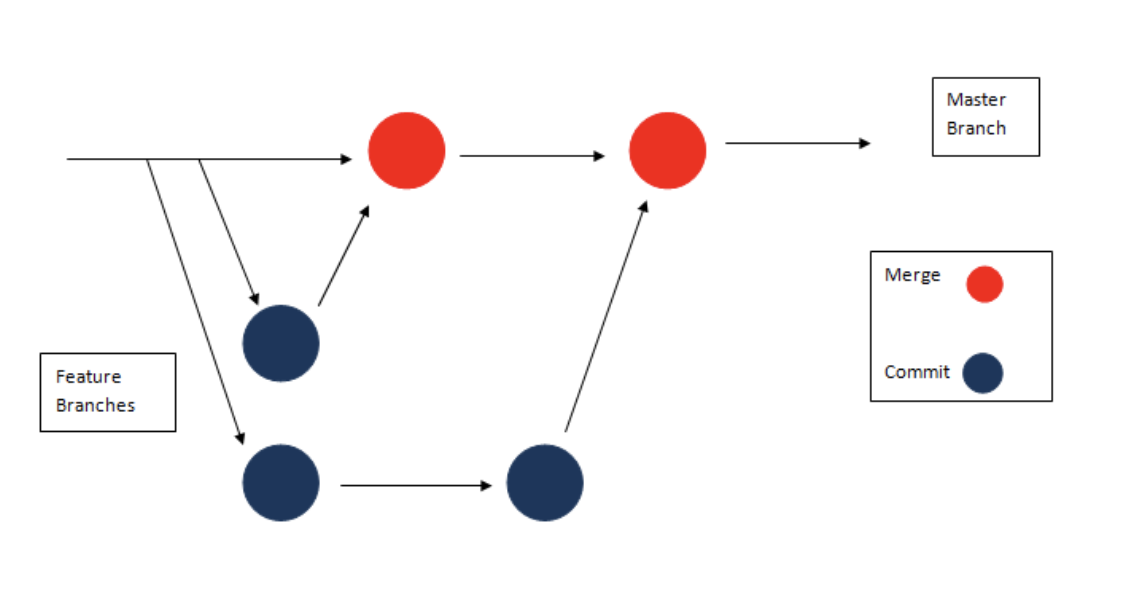
\includegraphics[scale=.69]{img/plan.png}
  \caption{Git Workflow Plan}
  \label{plan}
\end{figure}

\section{Proof of Concept Demonstration Plan}
While it would be ideal to create a shippable product by the end of the semester, this may not be possible as we have limited time. Here we will describe how we are going to structure the project and what features we will add, to make sure the group is able to reach our goals by the end of the semester. By the end of the semester our application should allow users to anonymously post questions to the class board(page in our webapp) and everyone following that class board should be able to see the question and upvote/reply to it. While there are many additional features we would like to add to make the user experience amazing, these are the core features we plan on completing by the end of the semester.For our first proof of concept demonstration we want our server side setup. We also aim to be able to post a string to a database and be able to pull it. For this demonstration we do not plan on have a user interface setup, just the core functionality.

\section{Technology}

\textbf{Programming Language:} JavaScript (TypeScript), HTML, CSS \\ 
\textbf{IDE:} JetBrains WebStorm\\
\textbf{Testing Framework:} Angular running on local host for testing purposes \\
\textbf{Document Generation:} Compodoc (Typedoc - depends on use of JS or TS) \\ 

Creating a Web-app built with Angular2 Framework requires the use of typescript (potentially also JavaScript), HTML and CSS. Due to past experiences that some of the team members have with the JetBrains WebStorm IDE, we will be using it for our project. It also has a terminal window that allows the developer to host the project with one simple command ("ng serve" while in root folder of project). In order to document this project, we will potentially need to use Compodoc or Typedoc, however no one person on our team is an expert on this yet and will require practical testing to determine which one to use. Testing Framework is quite simple, just host it locally as mentioned earlier and Angular2 updates live changes once it has been hosted. 

\section{Coding Style}
It is very important to make sure that the code in any code base is clear and conforms to a standard set of rules. This allows for ease in understanding of how the code actually works and communication between different coders. Naming and formatting will be done using regular conventions we learned in 2XA3, all our variables will be named using camel notation, classes will be named with capital. Regarding Whitespaces, there will be no whitespace after the end of a line. Indentation will be done using tabs. For Control structure, the rackets for things like loops and functions will begin at the end of the line not the next line. For control structure we will follow K\&R bracing style where the opening bracket is at the end of the first line and closing bracket is on it own line at the very end, aligned with the beginning of the first line. 

\section{Project Schedule}
Please click \href{run:../../ProjectSchedule/GanttChart.gan}{here} to open GanttChart.

\section{Project Review}

\end{document}


